\documentclass{beamer}

\usetheme{Madrid}
\usecolortheme{seahorse}
\setbeamertemplate{navigation symbols}{}
\setbeamerfont{title}{size=\large}

\usepackage{amsmath}
\usepackage{amssymb}
\usepackage{braket}
\usepackage{booktabs}
\usepackage{graphicx}
\usepackage{grffile}
\usepackage{tikz}
\usetikzlibrary{shapes.geometric,arrows.meta,positioning,fit}
\usepackage{xcolor}

\definecolor{nublue}{RGB}{0,50,120}
\setbeamercolor{title}{fg=white,bg=nublue}
\setbeamercolor{frametitle}{fg=white,bg=nublue}
\setbeamercolor{block title}{fg=white,bg=nublue}

%% Simple quantum wire macro
\newcommand{\qwire}[3]{% from x, to x, at y
  \draw[thick] (#1,#3) -- (#2,#3);
}
\newcommand{\qgate}[3]{% x, y, label
  \node[draw,thick,minimum width=1.2em,minimum height=1.2em,fill=white] at (#1,#2) {\small #3};
}

%% ----------------------------------------------------------------
\title[ODE Discretization for VQLS]{Discretizing ODE for Quantum Computers}
\author[A. Akimshe]{Adilet Akimshe\texorpdfstring{\\[4pt]}{ }
  {\small Advisor: Alejandro Javier Castro\texorpdfstring{\quad}{ }
         Second Reader: Adilet Otemissov}}
\institute[Dept.\ of Math, NU]{Department of Mathematics, Nazarbayev University}
\date{April 2026}
%% ----------------------------------------------------------------

\begin{document}

\begin{frame}
  \titlepage
\end{frame}

%% ----------------------------------------------------------------
\begin{frame}{Outline}
  \tableofcontents
\end{frame}

%% ----------------------------------------------------------------
\section{Motivation}

\begin{frame}[shrink=15]{Quantum Computing: From Labs to Industry}

  \begin{columns}[T]
    \begin{column}{0.48\textwidth}
      \begin{center}
        \includegraphics[width=\linewidth,height=0.50\textheight,keepaspectratio]{{google quantum computer}.jpg}\\[4pt]
        {\scriptsize Google Willow quantum processor:\\
        surpassed classical supercomputers on benchmark tasks}
      \end{center}
    \end{column}
    \begin{column}{0.48\textwidth}
      \begin{center}
        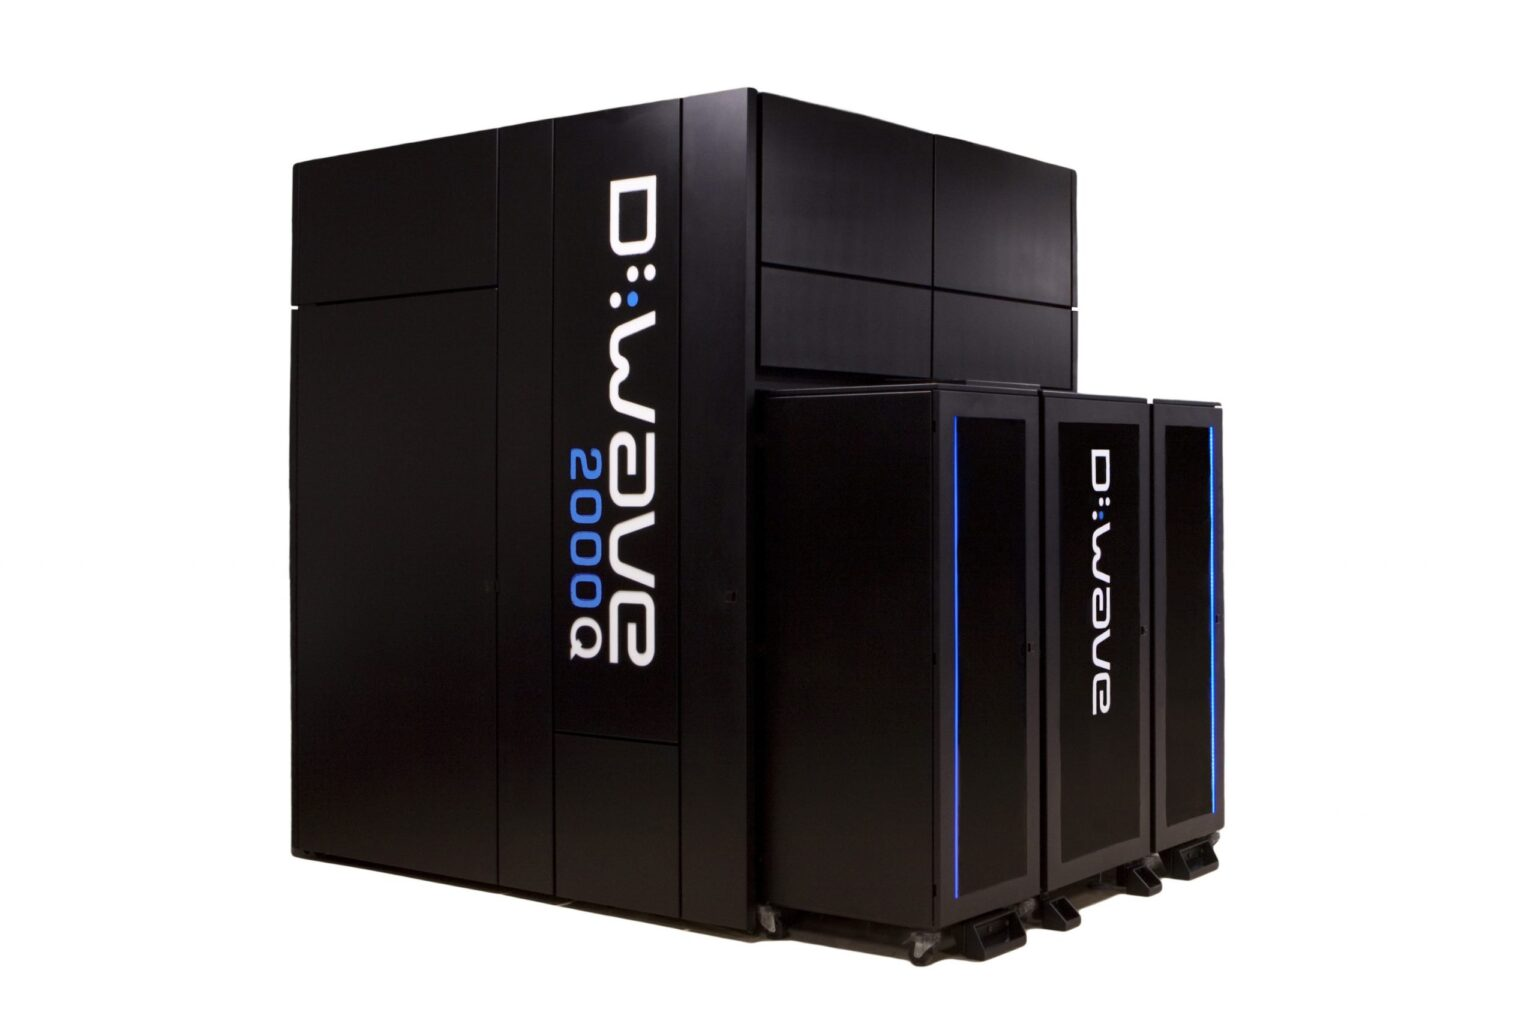
\includegraphics[width=\linewidth,height=0.50\textheight,keepaspectratio]{dwave.jpeg}\\[4pt]
        {\scriptsize D-Wave quantum annealer:\\
        commercial quantum computing}
      \end{center}
    \end{column}
  \end{columns}

  \vspace{4pt}
  \begin{block}{Quantum "arms race"}
    \textbf{Google, IBM, Microsoft, IonQ, D-Wave} — quantum hardware is
    advancing rapidly. Intermediary quantum algorithms are needed \emph{now} to make use
    of near-term noisy devices before full fault-tolerance arrives. Whoever gets it first will be filthy rich.
  \end{block}
\end{frame}


%% ----------------------------------------------------------------

\begin{frame}{Why Should Anyone Care?}

  \begin{columns}[T]
    \begin{column}{0.56\textwidth}
      \small
      \textbf{The big picture}
      \begin{itemize}\setlength\itemsep{2pt}
        \item Many scientific problems reduce to solving \emph{linear systems}
              $A\mathbf{x} = \mathbf{b}$
        \item Classical cost: $O(N^3)$ (Gaussian) or $O(N^2)$ (iterative)
              — expensive for large $N$
        \item \textbf{HHL quantum algorithm}: $O(\log N)$ depth —
              exponential speedup in $N$, but requires tomorrow's fault-tolerant quantum computers
        \item \textbf{VQLS quantum algorithm}: runs on near-term devices, but has conditions on the matrix $A$ (e.g.\ must be sparse in the Pauli basis)
      \end{itemize}

    \end{column}
    \begin{column}{0.40\textwidth}
      \begin{center}
        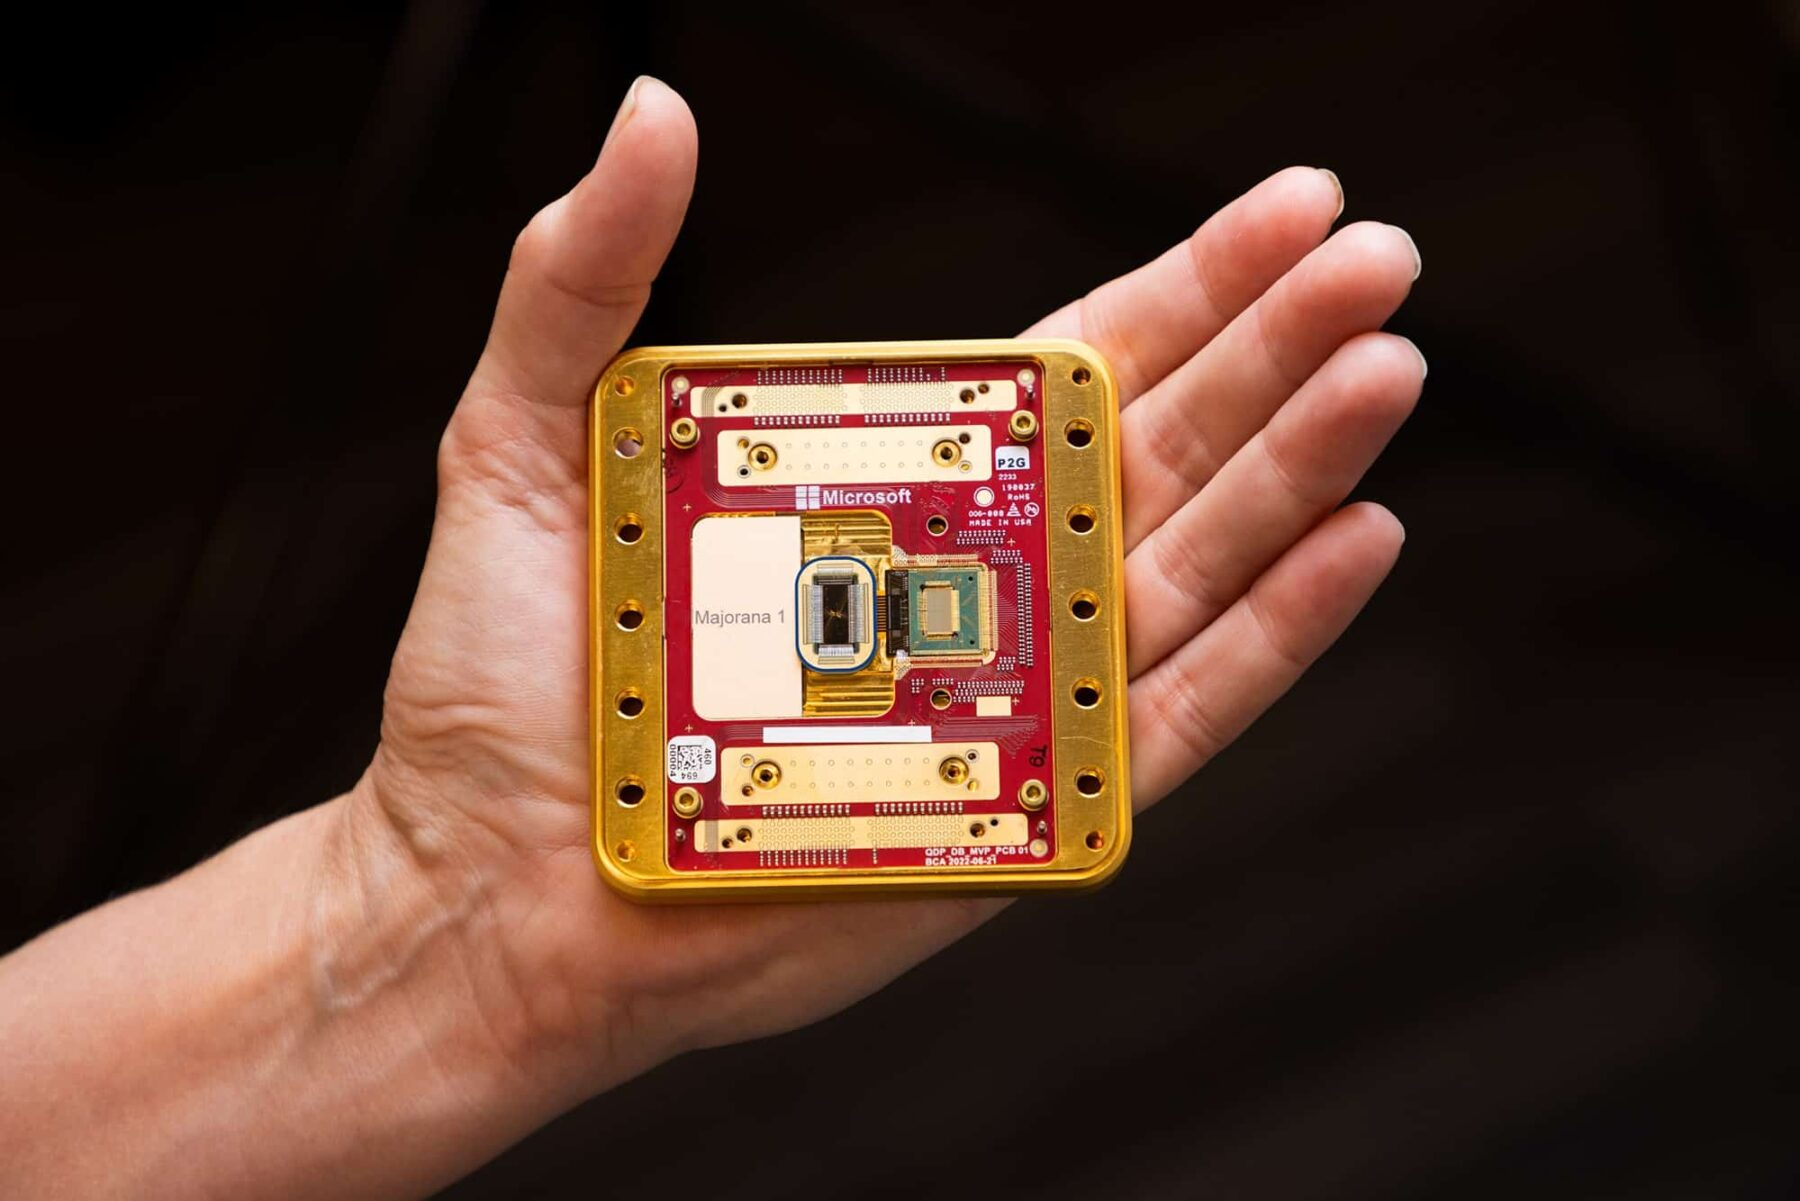
\includegraphics[width=\linewidth,height=0.62\textheight,keepaspectratio]{Majorana.jpg}\\[2pt]
        {\scriptsize Microsoft Majorana 1 chip (2025)}
      \end{center}
    \end{column}
  \end{columns}
\end{frame}

%% ----------------------------------------------------------------
\begin{frame}{Simulation vs.\ Real Quantum Hardware}

  \begin{columns}[T]
    \begin{column}{0.48\textwidth}
      \textbf{Classical (no quantum) simulation}
      \begin{itemize}\setlength\itemsep{3pt}
        \item Runs on CPU/GPU — exact, no noise
        \item Memory requirement doubles with every qubit added
        \item[$\Rightarrow$] Feasible only up to ${\sim}50$ qubits
      \end{itemize}

      \vspace{6pt}
      \emph{Our experiments use PennyLane's} \texttt{lightning.qubit} \emph{simulator
      — exact but expensive at $N=16$.}
    \end{column}
    \begin{column}{0.48\textwidth}
      \textbf{Real quantum hardware}
      \begin{itemize}\setlength\itemsep{3pt}
        \item Operates on physical qubits — inherently noisy
        \item Gate errors, decoherence, measurement noise
        \item \textbf{NISQ era:} 50--1000 noisy qubits today
      \end{itemize}

      \vspace{6pt}
      \begin{block}{Why simulate at all?}
        Simulation lets us \emph{validate} algorithms cheaply before
        running on expensive quantum hardware.
      \end{block}
    \end{column}
  \end{columns}
\end{frame}


%% ----------------------------------------------------------------
\section{Background}


%% ----------------------------------------------------------------
\begin{frame}{Variational Quantum Linear Solver (VQLS)}

  \begin{columns}
    \begin{column}{0.52\textwidth}
      \textbf{Goal:} solve $A\ket{x} = \ket{b}$ on a NISQ device.

      \vspace{6pt}
      \textbf{Algorithm loop:}
      \begin{enumerate}
        \item Prepare ansatz $\ket{\psi(\boldsymbol\theta)}=V(\boldsymbol\theta)\ket{0}$
        \item Evaluate cost $C(\boldsymbol\theta)=1-\tfrac{|\langle b|A|\psi\rangle|^2}
              {\langle\psi|A^\dagger A|\psi\rangle}$
        \item Update $\boldsymbol\theta$ by gradient descent
        \item Repeat until $C\approx 0$
      \end{enumerate}

      \vspace{6pt}
      % Hardware-efficient ansatz diagram (manual)
      \begin{center}
      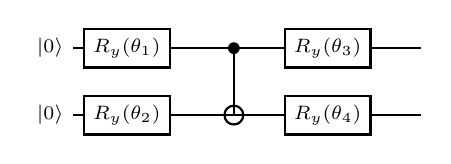
\begin{tikzpicture}[scale=0.85,
        gate/.style={draw,thick,minimum width=1.6em,minimum height=1.4em,fill=white,font=\scriptsize}
      ]
        \draw[thick](0,1)--(5.2,1); \draw[thick](0,0)--(5.2,0);
        \node[left,font=\scriptsize] at (0,1) {$|0\rangle$};
        \node[left,font=\scriptsize] at (0,0) {$|0\rangle$};
        \node[gate] at (0.8,1) {$R_y(\theta_1)$};
        \node[gate] at (0.8,0) {$R_y(\theta_2)$};
        % CNOT
        \fill (2.4,1) circle (2.5pt);
        \draw[thick](2.4,1)--(2.4,0);
        \draw[thick](2.4,0) circle (4pt);
        \draw[thick](2.4,0)+(0,4pt)--(2.4,0)+(-4pt,0pt);
        \draw[thick](2.4,0)+(0,4pt)--(2.4,0)+(4pt,0pt);
        \node[gate] at (3.8,1) {$R_y(\theta_3)$};
        \node[gate] at (3.8,0) {$R_y(\theta_4)$};
      \end{tikzpicture}
      \vspace{1pt}
      {\scriptsize Hardware-efficient ansatz (2 qubits)}
      \end{center}
    \end{column}
    \begin{column}{0.44\textwidth}
      \begin{block}{Analogy: supervised ML}
        {\footnotesize\renewcommand{\arraystretch}{1.05}%
        \begin{tabular}{ll}
          ML & VQLS \\ \hline
          Neural net & Quantum circuit \\
          Weights $\boldsymbol\theta$ & Gate angles \\
          Loss & Cost $C$ \\
          SGD step & Gradient step \\
          Forward pass & Circuit eval.
        \end{tabular}}
      \end{block}

      \vspace{4pt}
      \textbf{Two bottlenecks:}
      \begin{enumerate}
        \item Circuit overhead: $O(L^2 n)$ circuits/step
        \item Ansatz expressibility
      \end{enumerate}
      \smallskip
      Our work attacks \textbf{bottleneck 1}.
    \end{column}
  \end{columns}
\end{frame}

%% ----------------------------------------------------------------
\begin{frame}{Pauli Strings}

  \textbf{Pauli matrices}:
  \[
    I = \begin{pmatrix}1&0\\0&1\end{pmatrix},\quad
    X = \begin{pmatrix}0&1\\1&0\end{pmatrix},\quad
    Y = \begin{pmatrix}0&-i\\i&0\end{pmatrix},\quad
    Z = \begin{pmatrix}1&0\\0&-1\end{pmatrix}
  \]

  \textbf{Pauli strings} — tensor products of these matrices. They form an orthogonal basis for
  \emph{all} $2^n\times 2^n$ matrices. So any matrix $A$ decomposes as
  \[
    A \;=\; \sum_{P} c_P\, P, \qquad c_P = \tfrac{1}{2^n}\operatorname{Tr}(A\,P).
  \]

\end{frame}

%% ----------------------------------------------------------------
\begin{frame}[shrink=5]{Pauli Strings — Concrete Example}

  \begin{columns}[T]
    \begin{column}{0.50\textwidth}
      \textbf{Matrix} (1 qubit, basis $\{I,X,Y,Z\}$):
      \[
        A = \begin{pmatrix}3 & 1 \\ 1 & 1\end{pmatrix}
      \]
      \textbf{Coefficients} $c_P = \tfrac{1}{2}\operatorname{Tr}(AP)$:
      \[
        c_I=2,\quad c_X=1,\quad c_Y=0,\quad c_Z=1.
      \]
    \end{column}
    \begin{column}{0.46\textwidth}
      \textbf{Result — 3 nonzero Pauli strings:}
      \[ A \;=\; 2I + X + Z \]
      One can verify directly: $2I+X+Z = \begin{pmatrix}3&1\\1&1\end{pmatrix}\checkmark$
      \begin{block}{Why this matters for VQLS}
        \small One circuit per Pauli term: 3 circuits here.
        $Y$ dropped out — fewer nonzero $c_P$ means faster VQLS.
      \end{block}
    \end{column}
  \end{columns}
\end{frame}

%% ----------------------------------------------------------------
\begin{frame}{Collocation Discretization — Simple Example}

  \textbf{Problem:} $u'' = 0$, $u(0)=0$, $u(1)=1$. \;
  \emph{Exact solution: $u(t)=t$.}

  \vspace{4pt}
  \textbf{Spectral collocation} ($N=4$, monomial basis $\{1,t,t^2,t^3\}$):
  \begin{enumerate}
    \item Nodes: boundaries $t=0,1$ and interior (equally spaced) points $t=\tfrac{1}{3},\tfrac{2}{3}$
    \item Write $u(t)\approx c_0+c_1 t+c_2 t^2+c_3 t^3$
    \item Enforce BCs at rows 0--1; enforce $u''=0$ at rows 2--3
  \end{enumerate}

  \[
    \underbrace{\begin{pmatrix}
      1 & 0 & 0 & 0 \\
      1 & 1 & 1 & 1 \\
      0 & 0 & 2 & 2 \\
      0 & 0 & 2 & 4
    \end{pmatrix}}_{A_{\rm mono}}
    \begin{pmatrix}c_0\\c_1\\c_2\\c_3\end{pmatrix}
    = \begin{pmatrix}0\\1\\0\\0\end{pmatrix}
  \]

  \vspace{2pt}
  \begin{alertblock}{}
    How many Pauli strings does $A_{\rm mono}$ decompose into?
  \end{alertblock}
\end{frame}

%% ----------------------------------------------------------------
\begin{frame}{$A_{\rm mono}$ Decomposes into All 16 Pauli Strings}

  \begin{columns}[T]
    \begin{column}{0.38\textwidth}
      Recall $A_{\rm mono}$ for $u''=0$ on $[0,1]$:
      \[
        A_{\rm mono} = \begin{pmatrix}
          1&0&0&0\\1&1&1&1\\0&0&2&2\\0&0&2&4
        \end{pmatrix}
      \]
      Using $c_P = \tfrac{1}{4}\operatorname{Tr}(A_{\rm mono}\,P)$,
      \emph{every} 2-qubit Pauli string has a nonzero coefficient:
    \end{column}
    \begin{column}{0.58\textwidth}
      \renewcommand{\arraystretch}{1.05}
      \begin{center}
      \footnotesize
      \begin{tabular}{cc|cc|cc|cc}
        \toprule
        $P$ & $c_P$ & $P$ & $c_P$ & $P$ & $c_P$ & $P$ & $c_P$ \\
        \midrule
        $II$ & $+2$       & $XI$ & $+\tfrac{1}{4}$  & $YI$ & $+\tfrac{1}{4}$  & $ZI$ & $-1$       \\
        $IX$ & $+\tfrac{5}{4}$  & $XX$ & $+\tfrac{1}{4}$  & $YX$ & $+\tfrac{1}{4}$  & $ZX$ & $-\tfrac{3}{4}$  \\
        $IY$ & $-\tfrac{1}{4}$  & $XY$ & $-\tfrac{1}{4}$  & $YY$ & $+\tfrac{1}{4}$  & $ZY$ & $-\tfrac{1}{4}$  \\
        $IZ$ & $-\tfrac{1}{2}$  & $XZ$ & $-\tfrac{1}{4}$  & $YZ$ & $-\tfrac{1}{4}$  & $ZZ$ & $+\tfrac{1}{2}$  \\
        \bottomrule
      \end{tabular}
      \end{center}

      \vspace{4pt}
      \begin{alertblock}{Cost for VQLS}
        \small $L{=}16$ terms $\Rightarrow$ \textbf{768} circuits/step.\\
        Fewer $c_P$ $\Rightarrow$ faster VQLS.
      \end{alertblock}
    \end{column}
  \end{columns}
\end{frame}

%% ----------------------------------------------------------------
\begin{frame}{From Pauli Overhead to Basis Change}

  \begin{columns}[T]
    \begin{column}{0.48\textwidth}
      \textbf{The cost bottleneck}

      VQLS costs $L^2(n+1)$ circuits/step, where $L$ = nonzero Pauli terms.
      With the monomial basis, $A_{\rm mono}$ gives $L=16 \Rightarrow \mathbf{768}$ circuits/step.

      \vspace{10pt}
      \textbf{Key observation}

      The polynomial basis is a \emph{free choice} —
      it changes $A$ but \textbf{not the solution} $u$. What if we choose a different basis to get a different $A$ with fewer nonzero Pauli terms?
    \end{column}
    \begin{column}{0.48\textwidth}

      \vspace{8pt}
      \begin{alertblock}{Our idea}
        Better basis $\;\Rightarrow\;$ less Paulis $\;\Rightarrow\;$ fewer circuits $\;\Rightarrow\;$ faster VQLS.
      \end{alertblock}
    \end{column}
  \end{columns}
\end{frame}

%% ----------------------------------------------------------------
\section{Main Results}

\begin{frame}[shrink=12]{The Basis-Change Identity}

  \begin{block}{Key observation}
    The collocation matrix in \emph{any} polynomial basis $\{\phi_j\}$ is
    \[
      A_C = A_{\rm mono}\, C^\top,
    \]
    where $C_{jk}$ = coefficient of $t^k$ in $\phi_j$.
    The physical solution $u$ is \textbf{independent of the basis choice.}
  \end{block}

  \vspace{8pt}
  \begin{columns}
    \begin{column}{0.5\textwidth}
      \textbf{Consequence:}
      \begin{itemize}
        \item $C = I$ gives the monomial basis (Case A) with up to $4^n$ Pauli strings
        \item Any invertible $C$ gives a valid discretization
        \item The Pauli coefficients of $A_C$ are \emph{linear} in the entries of $C$
        \item[$\Rightarrow$] \textbf{Finding the sparsest $A_C$ is a linear program}
      \end{itemize}
    \end{column}
    \begin{column}{0.46\textwidth}
      \begin{alertblock}{LP for Pauli minimization}
        \vspace{-4pt}
        \[
          \begin{aligned}
            &\min_{C,\,\mathbf{t}}\;\textstyle\sum_{P} t_P \\
            &\text{s.t.}\; |c_P(C)| \le t_P,\;\det C \neq 0
          \end{aligned}
        \]
        \vspace{-4pt}
        Each $c_P$ is linear in $C$: \textbf{linear program}.
      \end{alertblock}
    \end{column}
  \end{columns}
\end{frame}

%% ----------------------------------------------------------------
\begin{frame}[shrink=12]{Global LP vs.\ Monic LP}

  \begin{columns}
    \begin{column}{0.48\textwidth}
      \textbf{Global LP} — optimize all $N^2$ entries of $C$:
      \begin{itemize}
        \item Always finds $A^* = I_N$
        \item Only 1 Pauli string ($I^{\otimes n}$)
        \item \textcolor{red}{Problem:} $I_N \ket{x}=\ket{b}$ means $\ket{x}=\ket{b}$
              — trivially classical, \textbf{no quantum advantage}
      \end{itemize}
    \end{column}
    \begin{column}{0.48\textwidth}
      \textbf{Monic LP} — restrict $C$ to lower-triangular, unit diagonal:
      \[
        C = \begin{pmatrix}1&&&\\*&1&&\\*&*&1&\\*&*&*&1\end{pmatrix}
      \]
      \begin{itemize}
        \item Only $\tfrac{N(N-1)}{2}$ free variables
        \item $A^* \neq I_N$ — system stays \textcolor{nublue}{non-trivial}
        \item No extra normalization constraint needed
        \item Moderate but genuine Pauli reduction
      \end{itemize}
    \end{column}
  \end{columns}

  \vspace{6pt}
  \begin{block}{The monic LP is the principled middle ground}
    Reduces circuit overhead substantially while preserving a meaningful quantum computation.
  \end{block}
\end{frame}

%% ----------------------------------------------------------------
\begin{frame}{Results: Pauli String Counts}

  \begin{center}
  \renewcommand{\arraystretch}{1.3}
  \resizebox{\linewidth}{!}{%
  \begin{tabular}{lcccc}
    \toprule
    Experiment & $N$ & Case A & Monic LP & Global LP \\
    \midrule
    $u''=0$, $[0,1]$                    & 4 & 16 & \textbf{6}  & 1 \\
    $u''+u'+u=f$, $[-1,1]$             & 4 & 16 & \textbf{10} & 1 \\
    $u''+u'+u=f$, $[-1,1]$ (8-pt)      & 8 & 64 & \textbf{36} & 1 \\
    \bottomrule
  \end{tabular}}
  \end{center}

  \vspace{8pt}
  \begin{columns}
    \begin{column}{0.48\textwidth}
      \textbf{Hadamard tests per gradient step:}
      \renewcommand{\arraystretch}{1.2}
      \begin{center}
      \resizebox{\linewidth}{!}{\renewcommand{\arraystretch}{1.1}%
      \begin{tabular}{lccc}
        \toprule
        & Case A & Monic LP & Global LP \\
        \midrule
        $N=4$ & 768 & 108 & 3 \\
        $N=8$ & 16\,384 & 5\,184 & 4 \\
        \bottomrule
      \end{tabular}}
      \end{center}
    \end{column}
    \begin{column}{0.48\textwidth}
      \begin{block}{Key takeaway}
        \small Monic LP:\\
        $\mathbf{7\times}$ speedup at $N{=}4$,\\
        $\mathbf{3.2\times}$ at $N{=}8$.\\
        Problem stays non-trivial.
      \end{block}
    \end{column}
  \end{columns}
\end{frame}

%% ----------------------------------------------------------------
\begin{frame}[shrink=10]{Timing Comparison Across System Sizes}

  Wall-clock time per VQLS gradient step on a CPU simulator
  (PennyLane, \texttt{lightning.qubit}).

  \vspace{4pt}
  \begin{center}
  \renewcommand{\arraystretch}{1.2}
  \resizebox{\linewidth}{!}{%
  \begin{tabular}{lccccccc}
    \toprule
    Size & $n$ & \multicolumn{2}{c}{Case A (Monomial)} &
                 \multicolumn{2}{c}{Monic LP} &
                 \multicolumn{2}{c}{Global LP ($I_N$)} \\
    \cmidrule(lr){3-4}\cmidrule(lr){5-6}\cmidrule(lr){7-8}
         &   & Paulis & s/step & Paulis & s/step & Paulis & s/step \\
    \midrule
    $4\times 4$   & 2 & 16  & 17.2         & 6   & 1.3          & 1 & 0.05  \\
    $8\times 8$   & 3 & 64  & $\sim$240    & 36  & $\sim$75     & 1 & 0.11  \\
    $16\times 16$ & 4 & 256 & $>$3000\,*   & 112 & $\sim$920\,* & 1 & $\sim$0.3 \\
    \bottomrule
    \multicolumn{8}{l}{\footnotesize *Extrapolated from $N^4\log N$ scaling; Case~A at $N=16$ is not feasible on CPU.}
  \end{tabular}}
  \end{center}

  \vspace{4pt}
  \begin{columns}
    \begin{column}{0.48\textwidth}
      \textbf{Scaling:} Cost $\sim L^2 n \sim N^4 \log N$ \\
      Every doubling of $N$ increases Case A cost by ${\approx}16\times$.
    \end{column}
    \begin{column}{0.48\textwidth}
      \begin{alertblock}{LP speedup grows with problem size}
        $N=4$: ${\approx}13\times$ \quad
        $N=8$: ${\approx}3.2\times$ \\
        $N=16$: ${\approx}3.3\times$ (projected)
      \end{alertblock}
    \end{column}
  \end{columns}
\end{frame}

%% ----------------------------------------------------------------
\begin{frame}[shrink=10]{VQLS Cost Convergence — $N=4$ ($u''+u'+u=f$)}

  \begin{columns}[T]
    \begin{column}{0.62\textwidth}
      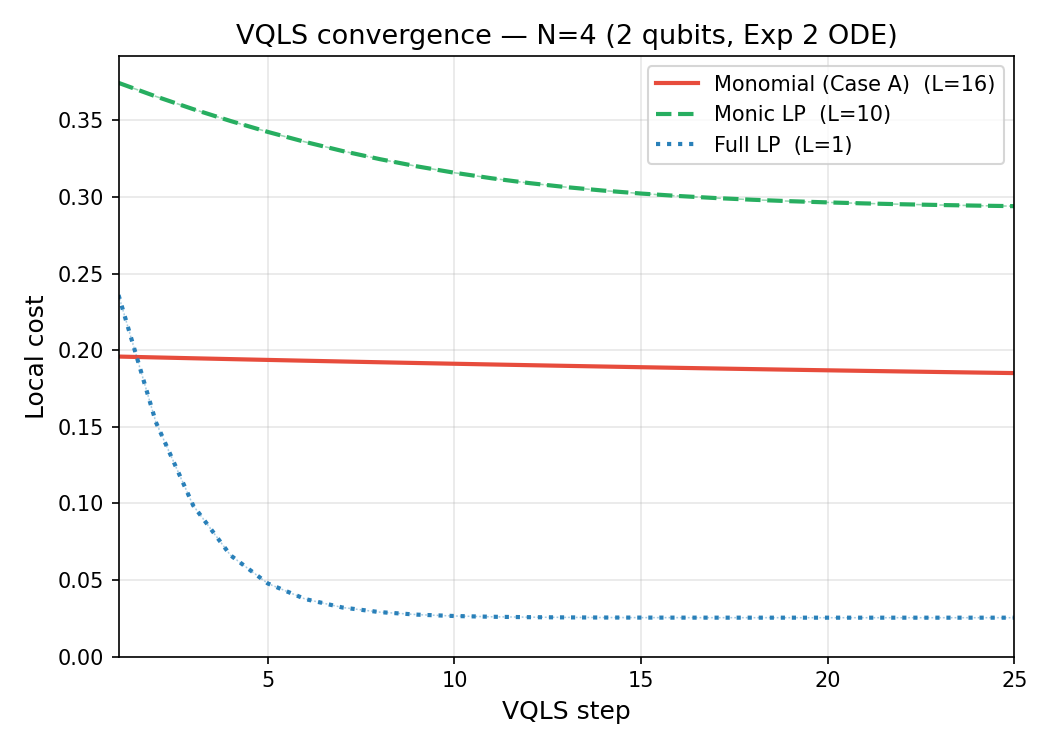
\includegraphics[width=\linewidth]{../plots/scaling_N4.png}
    \end{column}
    \begin{column}{0.35\textwidth}
      \small
      \textbf{Three bases, 25 gradient steps:}
      \begin{itemize}\setlength\itemsep{4pt}
        \item \textcolor{red}{\textbf{Case A}} ($L{=}16$): plateaus at $0.185$ immediately — too slow to escape
        \item \textcolor{teal}{\textbf{Monic LP}} ($L{=}10$): starts higher, slowly descends, plateaus at $0.294$
        \item \textcolor{blue}{\textbf{Full LP}} ($L{=}1$): drops to $0.025$ within 5 steps
      \end{itemize}

      \vspace{6pt}
      \begin{alertblock}{Key message}
        \small All three plateau — \emph{ansatz} is the binding limit.
        But Full LP reaches its plateau $\mathbf{237\times}$ faster.
      \end{alertblock}
    \end{column}
  \end{columns}
\end{frame}

%% ----------------------------------------------------------------
\begin{frame}{Convergence and Ansatz Limitation}

  \begin{columns}
    \begin{column}{0.50\textwidth}
      \textbf{Experiment 1} ($u''=0$, Global LP):
      \begin{itemize}
        \item Case A: cost $0.183$ after 20 steps (${\approx}344$\,s). Stuck.
        \item Global LP: converges to ${\approx}0$ in \textbf{13 steps} ($0.7$\,s)
      \end{itemize}

      \vspace{6pt}
      \textbf{Experiment 2} ($u''+u'+u=f$, Global LP):
      \begin{itemize}
        \item Case A: stuck at $0.187$ after 20 steps
        \item Global LP: drops to $0.025$ in \textbf{4 steps} ($0.25$\,s)
        \item Plateau at $0.025$ = ansatz expressibility limit
      \end{itemize}
    \end{column}
    \begin{column}{0.46\textwidth}
      \begin{block}{Two independent bottlenecks}
        \begin{enumerate}
          \item \textbf{Circuit overhead:} $O(L^2 n)$ Hadamard tests/step\\
                \emph{Fixed by LP preprocessing}
          \item \textbf{Ansatz expressibility:} circuit must represent $|x\rangle$\\
                \emph{Not affected by Pauli count — requires deeper ansatz}
        \end{enumerate}
      \end{block}
      \vspace{4pt}
      Both LP formulations share the same ansatz plateau —
      the overhead reduction is the sole benefit.
    \end{column}
  \end{columns}
\end{frame}

%% ----------------------------------------------------------------
\section{Conclusion}

\begin{frame}{Conclusion}
  \small
  \textbf{What we showed:}
  \begin{enumerate}\setlength\itemsep{3pt}
    \item The collocation matrix is freely adjustable via basis change
          without altering the solution — enabling LP-based Pauli minimization
    \item \textbf{Global LP} always finds $A^*=I_N$ (1 Pauli), but
          makes the problem classically trivial
    \item \textbf{Monic LP} finds a non-trivial $A^*$ with substantially fewer Paulis:
          $7\times$ speedup at $N=4$, growing with $N$
    \item Two independent VQLS bottlenecks: circuit overhead (cured by LP)
          and ansatz depth (separate issue)
  \end{enumerate}

  \vspace{6pt}
  \begin{block}{Practical recommendation}
    \small Apply \textbf{monic LP preprocessing} before VQLS on near-term hardware.
    Costs milliseconds of classical LP time; saves orders-of-magnitude in circuit evaluations.
  \end{block}
\end{frame}

%% ----------------------------------------------------------------
\begin{frame}{Future Work}

  \begin{columns}[T]
    \begin{column}{0.54\textwidth}
      \begin{block}{Open problems}
        \begin{itemize}\setlength\itemsep{4pt}
          \item \textbf{2D/3D PDEs:} joint basis-change LP over
                shared $B^\top$ — main open question
          \item \textbf{Node optimization:} Chebyshev/Legendre
                collocation nodes may reduce Paulis further
          \item \textbf{Deeper ansatz} to overcome expressibility plateau
          \item \textbf{Noise analysis} on real NISQ hardware
        \end{itemize}
      \end{block}
    \end{column}
    \begin{column}{0.42\textwidth}
      \begin{alertblock}{Key insight}
        In 1D, reducing Paulis removes quantum difficulty.
        \textbf{Multi-D PDEs} are the natural next target where
        quantum advantage may survive.
      \end{alertblock}
    \end{column}
  \end{columns}
\end{frame}

%% ----------------------------------------------------------------
\begin{frame}[plain]
  \vfill
  \begin{center}
    {\Large Thank you!}\\[12pt]
    {\large Questions?}\\[20pt]
    \hrule
    \vspace{8pt}
    {\small
    Adilet Akimshe \quad|\quad
    NU, Dept.\ of Mathematics\\[4pt]
    Advisor: Alejandro Javier Castro \quad
    Second Reader: Adilet Otemissov
    }
  \end{center}
  \vfill
\end{frame}

\end{document}
